\documentclass[12pt,a4paper]{article}
\usepackage[utf8]{inputenc}
\usepackage[T1]{fontenc}
\usepackage{lmodern}
\usepackage[margin=2.5cm]{geometry}
\usepackage{amsmath,amssymb}
\usepackage{graphicx}
\usepackage{float}
\usepackage{caption}
\usepackage{booktabs}
\usepackage{xcolor}
\usepackage{listings}
\usepackage{hyperref}

\renewcommand{\figurename}{pav}
\renewcommand{\tablename}{lentelė}
\DeclareCaptionLabelFormat{lt}{#2~#1}
\captionsetup{labelformat=lt, labelsep=period, font=small}

\lstset{
  language=Python, basicstyle=\ttfamily\footnotesize, breaklines=true,
  keywordstyle=\color{blue!70!black}, commentstyle=\color{green!40!black},
  stringstyle=\color{red!60!black}, frame=single, numbers=left,
  numberstyle=\tiny\color{gray}, showstringspaces=false, extendedchars=true,
  literate={ą}{{\k{a}}}1 {č}{{\v{c}}}1 {ę}{{\k{e}}}1 {ė}{{\.{e}}}1
           {į}{{\k{i}}}1 {š}{{\v{s}}}1 {ų}{{\k{u}}}1 {ū}{{\={u}}}1
           {ž}{{\v{z}}}1 {Ą}{{\k{A}}}1 {Č}{{\v{C}}}1 {Š}{{\v{S}}}1 {Ž}{{\v{Z}}}1
}

\title{II laboratorinis darbas\\[4pt]\large Paprastosios diferencialinės lygties pradinio uždavinio
skaitinis sprendimas\\ Variantas Nr.~9}
\author{Edvin Katenel, 1 grupė}
\date{2026 m. spalio 23 d.}

\begin{document}
\maketitle

\section*{Užduoties formulavimas}
Išspręskite Koši uždavinį
\[
  \begin{cases}
    \dfrac{du}{dx}=f(x,u)=x^2\cos(u-x),\\[6pt]
    u(0)=u_0,
  \end{cases}
  \qquad 0\le x\le 1,
\]
taikydami 4-pakopį Rungės--Kuto metodą ir antrąjį metodą Nr.~3 -- dvipakopį Rungės--Kuto metodą,
kai $\sigma=0.5$. Pasirinkta pradinė sąlyga $u(0)=0$, skaičiuota su žingsniais $\tau=0.1$ ir
$\tau=0.05$. Paklaidą intervale $(0,1]$ įvertinkite Rungės metodu. Uždavinį taip pat išspręskite
kompiuterine funkcija, kurioje naudojamas Rungės--Kuto metodas, ir grafiškai palyginkite rezultatus:
(a) metodas tas pats, skiriasi žingsnis; (b) žingsnis tas pats, skiriasi metodas.

Programa parašyta \texttt{Python} kalba (\texttt{NumPy}, \texttt{Matplotlib}). Kaip kompiuterinė
funkcija naudota \texttt{solve\_ivp} iš bibliotekos \texttt{scipy.integrate} su metodu
\texttt{RK45} (Dormando--Princo įterptinis Rungės--Kuto metodas su automatiniu žingsnio
parinkimu), tolerancijos $\texttt{rtol}=10^{-12}$, $\texttt{atol}=10^{-14}$. Lygtis nėra nei
tiesinė, nei su atskiriamaisiais kintamaisiais, jos analitinio sprendinio neturime, todėl
\texttt{solve\_ivp} sprendinys laikomas etaloniniu $u(x)$. Programos kodas pateiktas priede.

Tinklas: $x_i=i\tau$, $i=0,1,\dots,N$, $N=1/\tau$; $y_i\approx u(x_i)$, $y_0=u_0$.

%=====================================================================
\section{Taikyti metodai}

\subsection{4-pakopis Rungės--Kuto metodas ($p=4$)}
\[
\begin{aligned}
  k_1&=f(x_i,\,y_i), &
  k_2&=f\!\left(x_i+\tfrac{\tau}{2},\,y_i+\tfrac{\tau}{2}k_1\right),\\
  k_3&=f\!\left(x_i+\tfrac{\tau}{2},\,y_i+\tfrac{\tau}{2}k_2\right), &
  k_4&=f(x_i+\tau,\,y_i+\tau k_3),
\end{aligned}
\]
\[
  y_{i+1}=y_i+\frac{\tau}{6}\,(k_1+2k_2+2k_3+k_4).
\]
\emph{Geometrinė interpretacija:} krypties koeficientas apskaičiuojamas keturiuose taškuose
(intervalo pradžioje, du kartus viduryje ir gale), o žingsnis daromas pagal jų svertinį vidurkį
su svoriais $1:2:2:1$ (kaip Simpsono formulėje). Lokalioji paklaida $O(\tau^5)$, globalioji --
$O(\tau^4)$.

\subsection{Dvipakopis Rungės--Kuto metodas, $\sigma=0.5$ ($p=2$)}
Bendroji dvipakopių metodų šeima:
\[
  y_{i+1}=y_i+\tau\big[(1-\sigma)k_1+\sigma k_2\big],\qquad
  k_1=f(x_i,y_i),\quad
  k_2=f\!\left(x_i+\tfrac{\tau}{2\sigma},\,y_i+\tfrac{\tau}{2\sigma}k_1\right).
\]
Kai $\sigma=0.5$, gauname \textbf{prediktoriaus--korektoriaus (Hojno) metodą}:
\[
  \tilde y_{i+1}=y_i+\tau f(x_i,y_i)\quad\text{(prediktorius -- Eulerio žingsnis)},
\]
\[
  y_{i+1}=y_i+\frac{\tau}{2}\Big[f(x_i,y_i)+f(x_{i+1},\tilde y_{i+1})\Big]
  \quad\text{(korektorius -- trapecijų formulė)}.
\]
\emph{Geometrinė interpretacija:} pirmiausia Eulerio metodu (liestine) „nuspėjamas“ taškas
intervalo gale, tada žingsnis daromas pagal krypties koeficientų intervalo pradžioje ir gale
vidurkį. Globalioji paklaida $O(\tau^2)$.

\subsection{Paklaidos įvertis Rungės metodu}
\[
  |u(T)-y_\tau|\approx\frac{|y_{2\tau}-y_\tau|}{2^p-1},
\]
čia $y_\tau$ -- sprendinys su žingsniu $\tau=0.05$, $y_{2\tau}$ -- su žingsniu $2\tau=0.1$,
$p$ -- metodo tikslumo eilė ($2^p-1=15$ RK4 metodui ir $2^p-1=3$ dvipakopiam metodui).
Įvertis skaičiuotas visuose bendruose tinklų taškuose $T=0.1,0.2,\dots,1$.

%=====================================================================
\section{Rezultatai}

\begin{table}[H]
\centering\small
\caption{Skaitiniai sprendiniai tinklo taškuose, $u(0)=0$.}
\begin{tabular}{c|cc|cc|c}
\toprule
 & \multicolumn{2}{c|}{4-pakopis RK} & \multicolumn{2}{c|}{dvipakopis RK, $\sigma=0.5$} & \\
$x$ & $\tau=0.1$ & $\tau=0.05$ & $\tau=0.1$ & $\tau=0.05$ & \texttt{solve\_ivp} \\
\midrule
0.0 & 0.00000000 & 0.00000000 & 0.00000000 & 0.00000000 & 0.00000000\\
0.1 & 0.00033230 & 0.00033234 & 0.00049750 & 0.00037360 & 0.00033234\\
0.2 & 0.00263526 & 0.00263534 & 0.00295575 & 0.00271542 & 0.00263534\\
0.3 & 0.00876816 & 0.00876827 & 0.00922511 & 0.00888257 & 0.00876827\\
0.4 & 0.02039126 & 0.02039138 & 0.02095912 & 0.02053374 & 0.02039139\\
0.5 & 0.03891923 & 0.03891935 & 0.03956866 & 0.03908273 & 0.03891936\\
0.6 & 0.06552296 & 0.06552307 & 0.06622384 & 0.06570032 & 0.06552308\\
0.7 & 0.10117819 & 0.10117829 & 0.10190202 & 0.10136268 & 0.10117830\\
0.8 & 0.14675438 & 0.14675445 & 0.14747571 & 0.14694005 & 0.14675445\\
0.9 & 0.20313742 & 0.20313747 & 0.20383384 & 0.20331910 & 0.20313748\\
1.0 & 0.27138395 & 0.27138399 & 0.27203432 & 0.27155677 & 0.27138400\\
\bottomrule
\end{tabular}
\end{table}

\begin{table}[H]
\centering\small
\caption{Paklaidos įvertis Rungės metodu ($\tau=0.05$, $2\tau=0.1$) ir tikroji paklaida
$|u(x)-y_\tau|$, kai $u(x)$ -- \texttt{solve\_ivp} sprendinys.}
\begin{tabular}{c|cc|cc}
\toprule
 & \multicolumn{2}{c|}{4-pakopis RK ($p=4$)} & \multicolumn{2}{c}{dvipakopis RK, $\sigma=0.5$ ($p=2$)}\\
$x$ & Rungės įvertis & tikroji paklaida & Rungės įvertis & tikroji paklaida\\
\midrule
0.1 & $2.60\cdot10^{-9}$ & $2.57\cdot10^{-9}$ & $4.13\cdot10^{-5}$ & $4.13\cdot10^{-5}$\\
0.2 & $4.95\cdot10^{-9}$ & $4.86\cdot10^{-9}$ & $8.01\cdot10^{-5}$ & $8.01\cdot10^{-5}$\\
0.3 & $6.76\cdot10^{-9}$ & $6.60\cdot10^{-9}$ & $1.14\cdot10^{-4}$ & $1.14\cdot10^{-4}$\\
0.4 & $7.86\cdot10^{-9}$ & $7.63\cdot10^{-9}$ & $1.42\cdot10^{-4}$ & $1.42\cdot10^{-4}$\\
0.5 & $8.14\cdot10^{-9}$ & $7.87\cdot10^{-9}$ & $1.62\cdot10^{-4}$ & $1.63\cdot10^{-4}$\\
0.6 & $7.62\cdot10^{-9}$ & $7.32\cdot10^{-9}$ & $1.75\cdot10^{-4}$ & $1.77\cdot10^{-4}$\\
0.7 & $6.41\cdot10^{-9}$ & $6.11\cdot10^{-9}$ & $1.80\cdot10^{-4}$ & $1.84\cdot10^{-4}$\\
0.8 & $4.78\cdot10^{-9}$ & $4.50\cdot10^{-9}$ & $1.79\cdot10^{-4}$ & $1.86\cdot10^{-4}$\\
0.9 & $3.26\cdot10^{-9}$ & $3.01\cdot10^{-9}$ & $1.72\cdot10^{-4}$ & $1.82\cdot10^{-4}$\\
1.0 & $2.86\cdot10^{-9}$ & $2.63\cdot10^{-9}$ & $1.59\cdot10^{-4}$ & $1.73\cdot10^{-4}$\\
\midrule
$\max\limits_{(0,1]}$ & $8.14\cdot10^{-9}$ & $7.87\cdot10^{-9}$ & $1.80\cdot10^{-4}$ & $1.86\cdot10^{-4}$\\
\bottomrule
\end{tabular}
\end{table}

Rungės įvertis labai gerai sutampa su tikrąja paklaida, t.\,y. juo galima patikimai vertinti
tikslumą, nežinant tikslaus sprendinio. Taške $x=1$ sumažinus žingsnį perpus, RK4 metodo paklaida
sumažėjo nuo $4.55\cdot10^{-8}$ iki $2.63\cdot10^{-9}$ (apie $17$ kartų, teoriškai $2^4=16$), o
dvipakopio metodo -- nuo $6.50\cdot10^{-4}$ iki $1.73\cdot10^{-4}$ (apie $3.8$ karto, teoriškai
$2^2=4$). Tai patvirtina metodų tikslumo eiles $p=4$ ir $p=2$.

%=====================================================================
\section{Grafinis palyginimas}
Kiekviename paveiksle viršuje pavaizduoti sprendiniai (pilka storesnė linija --
\texttt{solve\_ivp}), apačioje -- paklaida $|y_i-u(x_i)|$ logaritminėje skalėje, nes viršutiniame
grafike kreivės praktiškai sutampa.

\subsection{(a) Metodas tas pats, skiriasi žingsnis}

\begin{figure}[H]
  \centering
  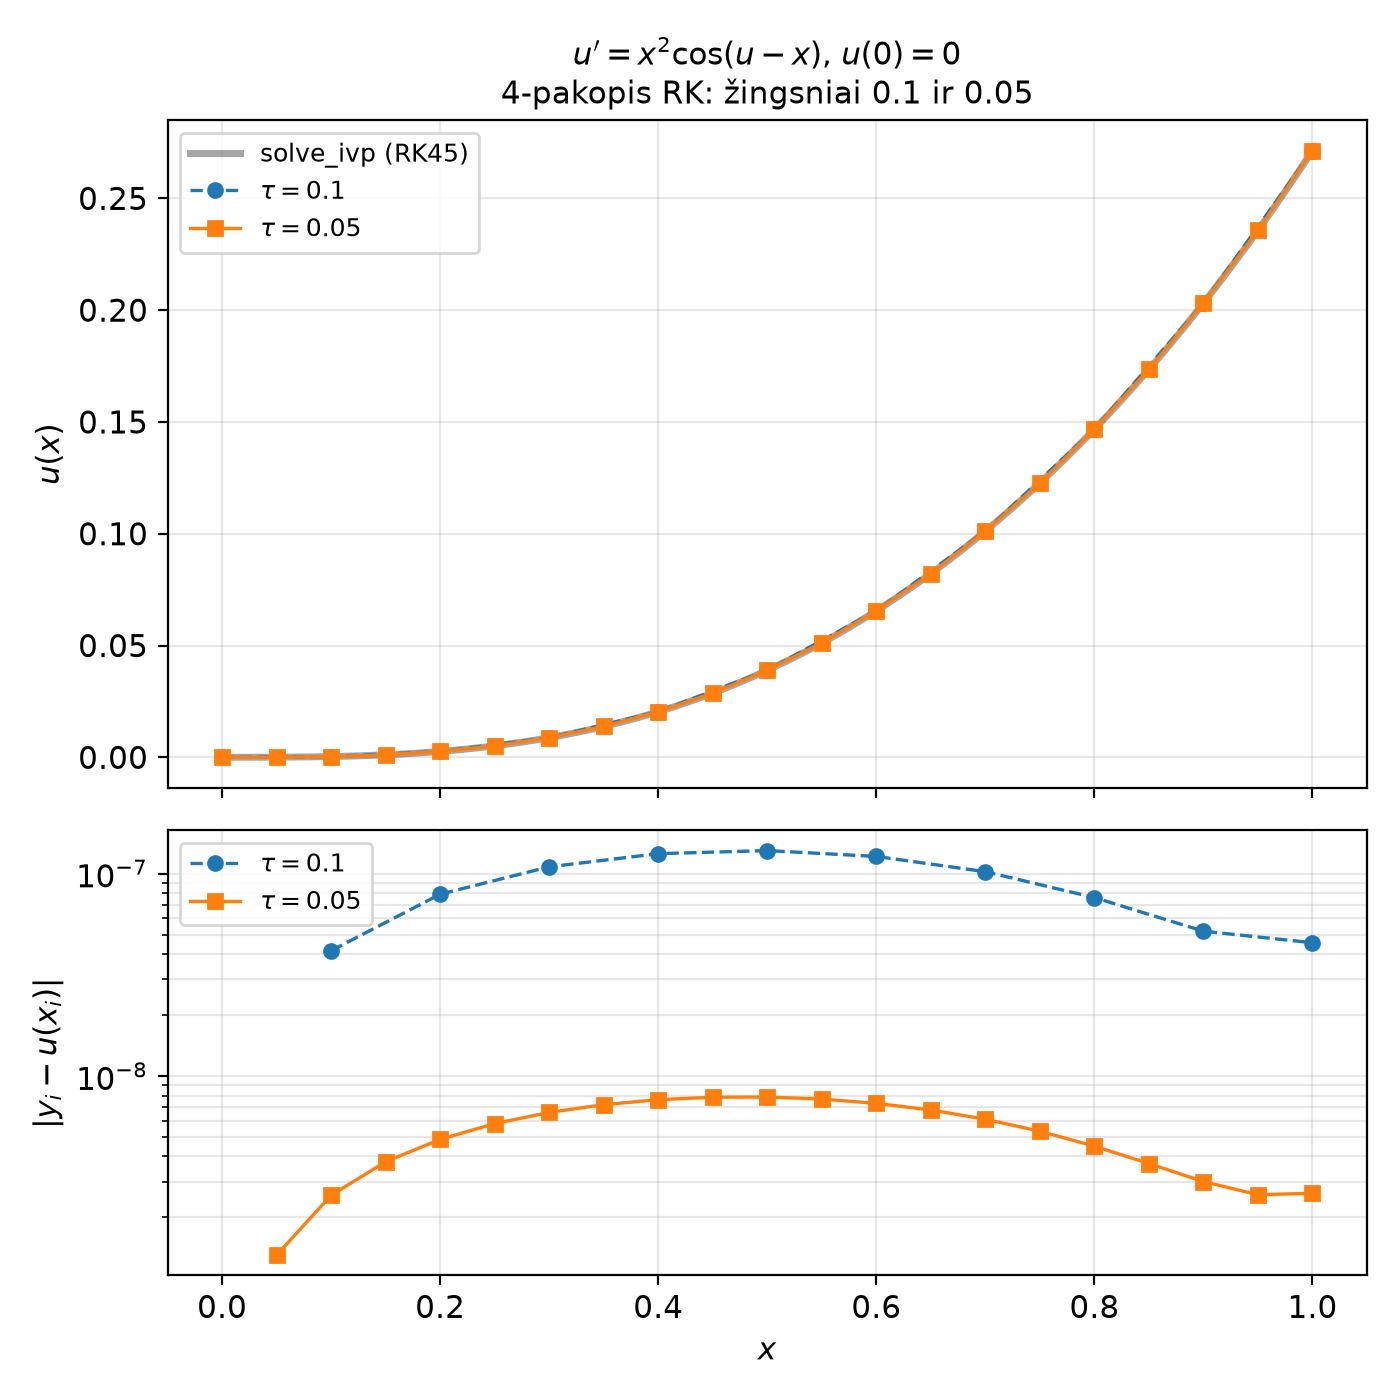
\includegraphics[width=0.5\textwidth]{fig_a_rk4.png}
  \caption{4-pakopis RK metodas su žingsniais $\tau=0.1$ ir $\tau=0.05$ bei \texttt{solve\_ivp}
  sprendinys. Paveikslėlyje matome, kad visos trys kreivės sutampa, o paklaida su $\tau=0.1$ yra
  apie $10^{-7}$, su $\tau=0.05$ -- apie $10^{-8}$--$10^{-9}$, t.\,y. apie 16 kartų mažesnė.
  Grafikas toks, nes RK4 metodo globalioji paklaida yra $O(\tau^4)$, todėl perpus sumažinus
  žingsnį paklaida sumažėja $2^4=16$ kartų.}
\end{figure}

\begin{figure}[H]
  \centering
  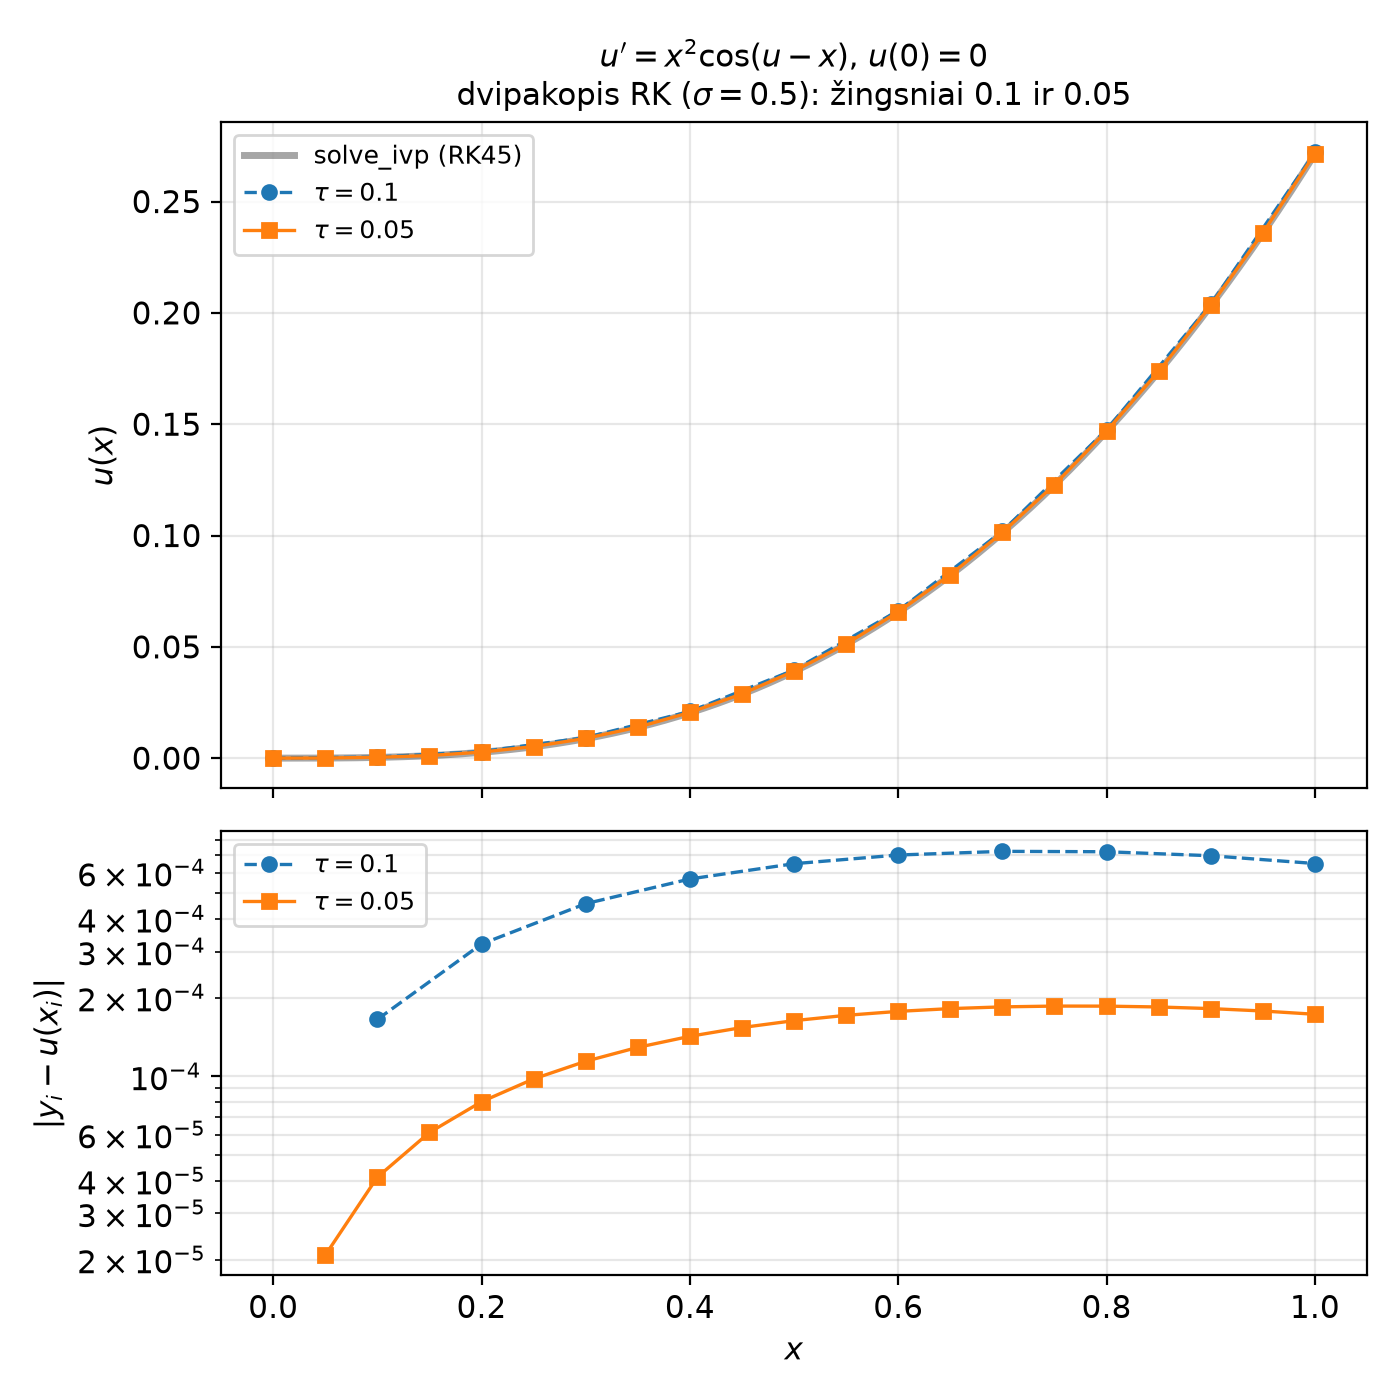
\includegraphics[width=0.5\textwidth]{fig_a_rk2.png}
  \caption{Dvipakopis RK metodas ($\sigma=0.5$) su žingsniais $\tau=0.1$ ir $\tau=0.05$ bei
  \texttt{solve\_ivp} sprendinys. Paveikslėlyje matome, kad skaitiniai sprendiniai yra šiek tiek
  virš tikslaus, paklaida auga ir apie $x\approx0.7$ nusistovi ties $7\cdot10^{-4}$ ($\tau=0.1$) ir
  $1.8\cdot10^{-4}$ ($\tau=0.05$). Grafikas toks, nes metodo globalioji paklaida yra $O(\tau^2)$ --
  perpus sumažinus žingsnį paklaida sumažėja apie 4 kartus, o kiekviename žingsnyje susidariusi
  lokalioji paklaida kaupiasi.}
\end{figure}

\subsection{(b) Žingsnis tas pats, skiriasi metodas}

\begin{figure}[H]
  \centering
  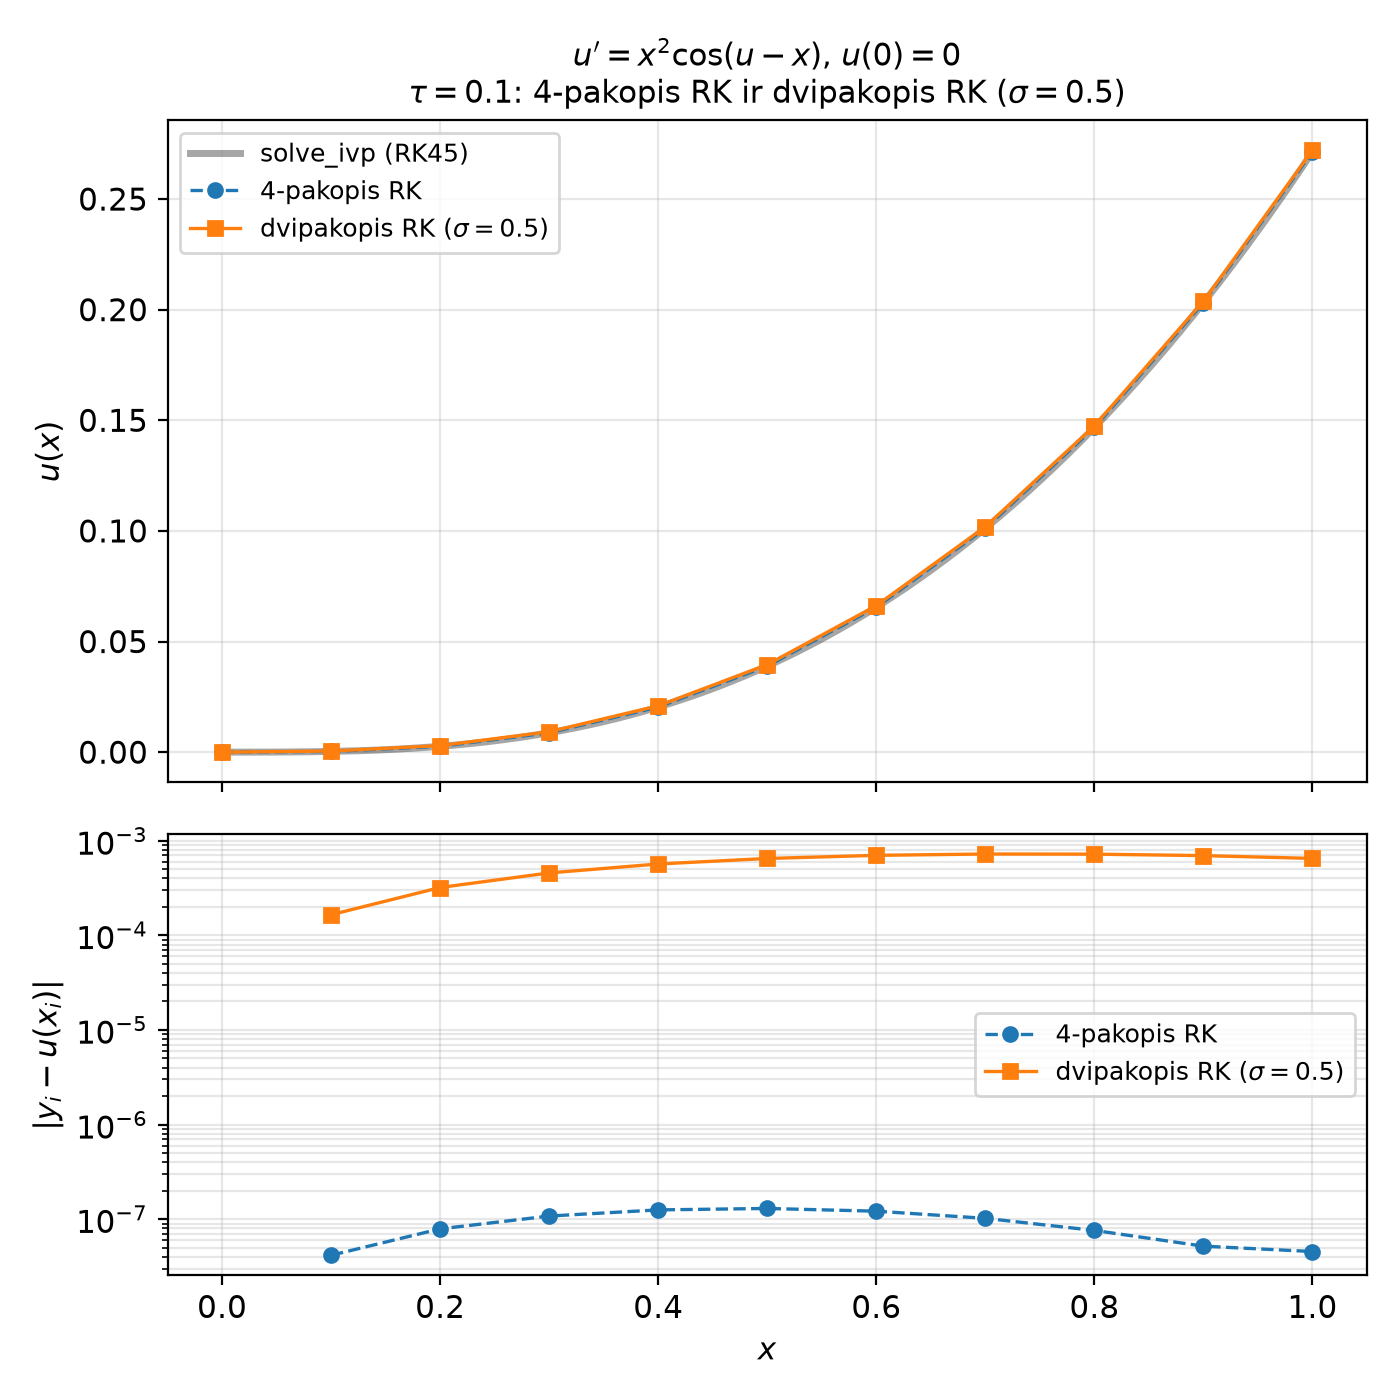
\includegraphics[width=0.5\textwidth]{fig_b_2tau.png}
  \caption{Žingsnis $\tau=0.1$: 4-pakopis ir dvipakopis RK metodai bei \texttt{solve\_ivp}.
  Paveikslėlyje matome, kad abu sprendiniai akimi sutampa su \texttt{solve\_ivp}, tačiau dvipakopio
  metodo paklaida ($\sim\!10^{-4}$--$10^{-3}$) yra kelis tūkstančius kartų didesnė nei RK4 ($\sim\!10^{-7}$).
  Grafikas toks, nes RK4 metodas kiekviename žingsnyje funkciją $f$ skaičiuoja 4 kartus ir yra
  ketvirtos eilės, o dvipakopis -- tik 2 kartus ir yra antros eilės.}
\end{figure}

\begin{figure}[H]
  \centering
  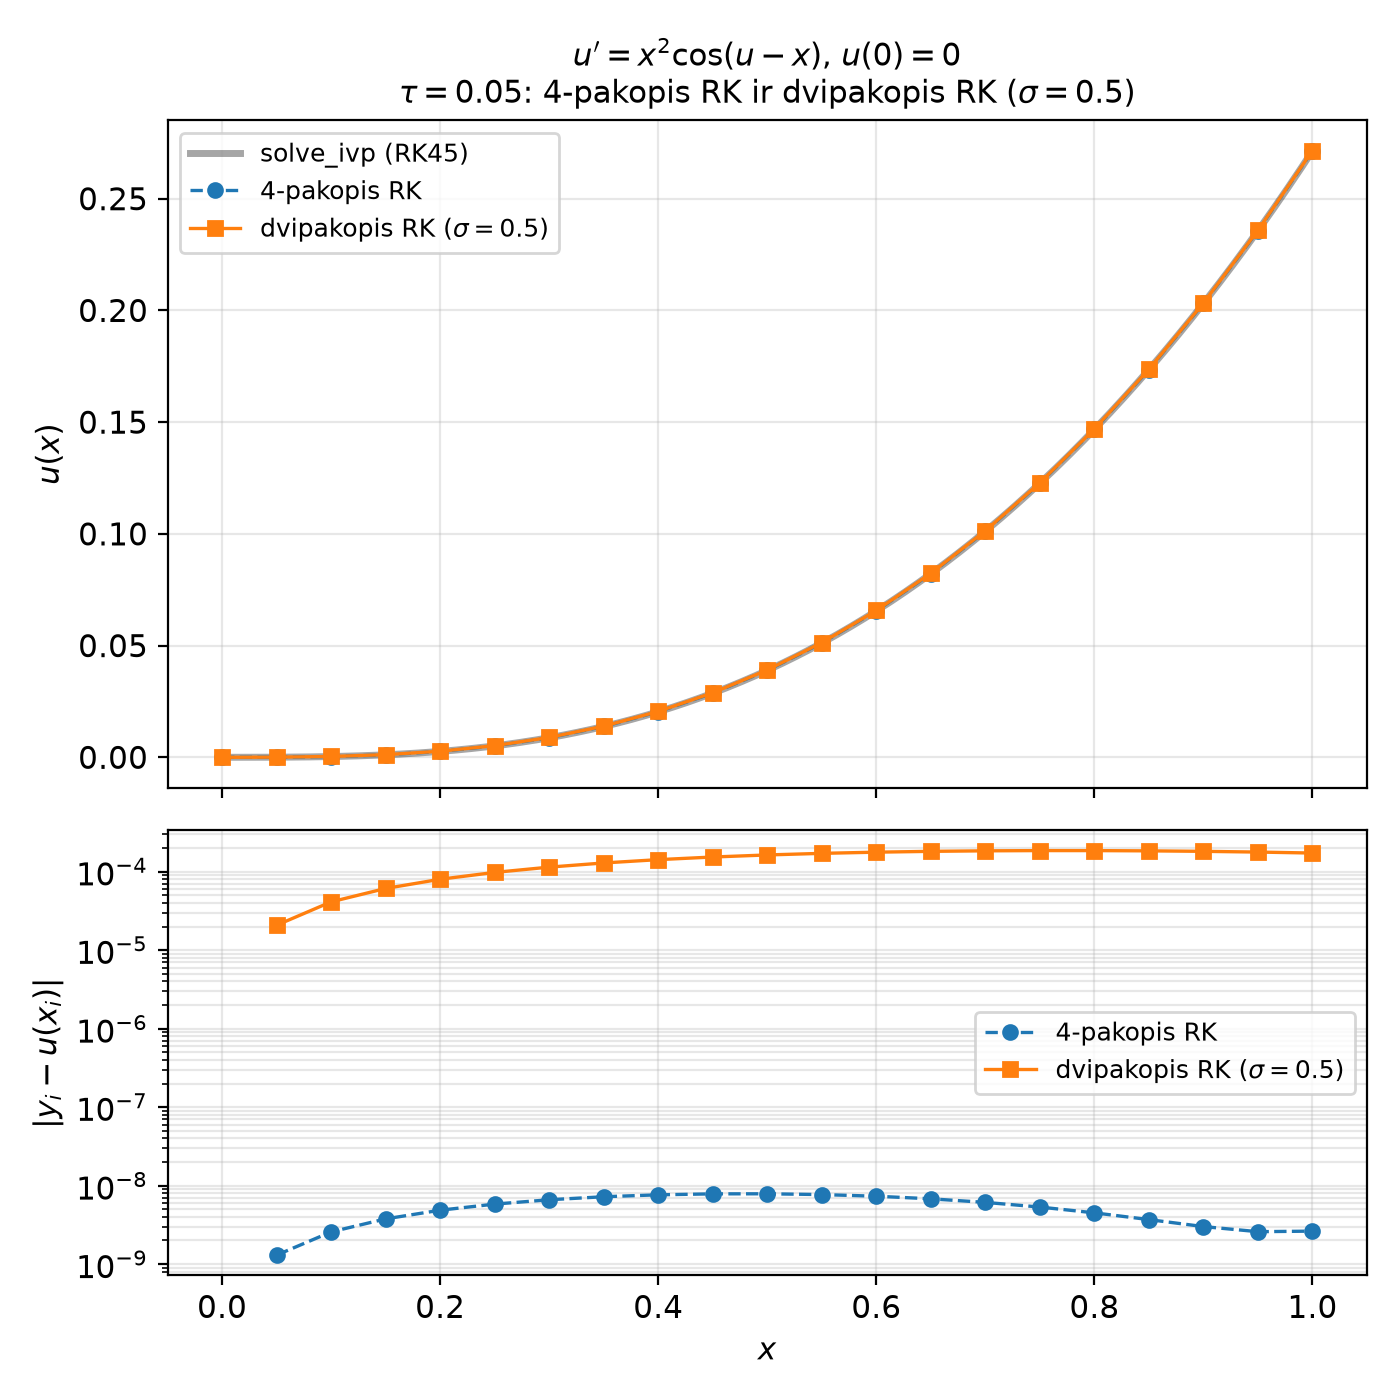
\includegraphics[width=0.5\textwidth]{fig_b_tau.png}
  \caption{Žingsnis $\tau=0.05$: 4-pakopis ir dvipakopis RK metodai bei \texttt{solve\_ivp}.
  Paveikslėlyje matome tą patį vaizdą kaip 3~pav., tik abiejų metodų paklaidos mažesnės, o
  atotrūkis tarp jų dar didesnis (dešimtys tūkstančių kartų). Grafikas toks, nes mažinant žingsnį
  aukštesnės eilės metodo paklaida mažėja greičiau ($\tau^4$ prieš $\tau^2$).}
\end{figure}

Sprendinio kreivė visuose paveiksluose prasideda horizontaliai ir lėtai kyla: kadangi $u(0)=0$, o
$f(0,u)=0$, pradžioje $u'\approx x^2$, todėl $u\approx x^3/3$; vėliau $\cos(u-x)<1$ šiek tiek
lėtina augimą, todėl $u(1)\approx0.2714<1/3$.

%=====================================================================
\section*{Išvados}
\begin{enumerate}
  \item Abu metodai ir \texttt{solve\_ivp} duoda tą patį sprendinį: $u(1)\approx0.271384$.
  \item 4-pakopis RK metodas daug tikslesnis: didžiausia paklaida intervale $(0,1]$ su $\tau=0.05$
        yra apie $8\cdot10^{-9}$, o dvipakopio metodo ($\sigma=0.5$) -- apie $1.9\cdot10^{-4}$.
  \item Perpus sumažinus žingsnį, paklaida sumažėja apie $2^p$ kartų (16 ir 4 kartus), kaip ir
        numato teorija.
  \item Rungės metodo įvertis praktiškai sutampa su tikrąja paklaida, todėl yra patikimas
        būdas vertinti paklaidą, kai tikslus sprendinys nežinomas.
\end{enumerate}

\newpage
\section*{Priedas. Programos kodas}
\lstinputlisting{lab2_var9.py}

\end{document}
